% Options for packages loaded elsewhere
\PassOptionsToPackage{unicode}{hyperref}
\PassOptionsToPackage{hyphens}{url}
%
\documentclass[
]{article}
\usepackage{lmodern}
\usepackage{amssymb,amsmath}
\usepackage{ifxetex,ifluatex}
\ifnum 0\ifxetex 1\fi\ifluatex 1\fi=0 % if pdftex
  \usepackage[T1]{fontenc}
  \usepackage[utf8]{inputenc}
  \usepackage{textcomp} % provide euro and other symbols
\else % if luatex or xetex
  \usepackage{unicode-math}
  \defaultfontfeatures{Scale=MatchLowercase}
  \defaultfontfeatures[\rmfamily]{Ligatures=TeX,Scale=1}
\fi
% Use upquote if available, for straight quotes in verbatim environments
\IfFileExists{upquote.sty}{\usepackage{upquote}}{}
\IfFileExists{microtype.sty}{% use microtype if available
  \usepackage[]{microtype}
  \UseMicrotypeSet[protrusion]{basicmath} % disable protrusion for tt fonts
}{}
\makeatletter
\@ifundefined{KOMAClassName}{% if non-KOMA class
  \IfFileExists{parskip.sty}{%
    \usepackage{parskip}
  }{% else
    \setlength{\parindent}{0pt}
    \setlength{\parskip}{6pt plus 2pt minus 1pt}}
}{% if KOMA class
  \KOMAoptions{parskip=half}}
\makeatother
\usepackage{xcolor}
\IfFileExists{xurl.sty}{\usepackage{xurl}}{} % add URL line breaks if available
\IfFileExists{bookmark.sty}{\usepackage{bookmark}}{\usepackage{hyperref}}
\hypersetup{
  pdftitle={Lab},
  hidelinks,
  pdfcreator={LaTeX via pandoc}}
\urlstyle{same} % disable monospaced font for URLs
\usepackage[margin=1in]{geometry}
\usepackage{color}
\usepackage{fancyvrb}
\newcommand{\VerbBar}{|}
\newcommand{\VERB}{\Verb[commandchars=\\\{\}]}
\DefineVerbatimEnvironment{Highlighting}{Verbatim}{commandchars=\\\{\}}
% Add ',fontsize=\small' for more characters per line
\usepackage{framed}
\definecolor{shadecolor}{RGB}{248,248,248}
\newenvironment{Shaded}{\begin{snugshade}}{\end{snugshade}}
\newcommand{\AlertTok}[1]{\textcolor[rgb]{0.94,0.16,0.16}{#1}}
\newcommand{\AnnotationTok}[1]{\textcolor[rgb]{0.56,0.35,0.01}{\textbf{\textit{#1}}}}
\newcommand{\AttributeTok}[1]{\textcolor[rgb]{0.77,0.63,0.00}{#1}}
\newcommand{\BaseNTok}[1]{\textcolor[rgb]{0.00,0.00,0.81}{#1}}
\newcommand{\BuiltInTok}[1]{#1}
\newcommand{\CharTok}[1]{\textcolor[rgb]{0.31,0.60,0.02}{#1}}
\newcommand{\CommentTok}[1]{\textcolor[rgb]{0.56,0.35,0.01}{\textit{#1}}}
\newcommand{\CommentVarTok}[1]{\textcolor[rgb]{0.56,0.35,0.01}{\textbf{\textit{#1}}}}
\newcommand{\ConstantTok}[1]{\textcolor[rgb]{0.00,0.00,0.00}{#1}}
\newcommand{\ControlFlowTok}[1]{\textcolor[rgb]{0.13,0.29,0.53}{\textbf{#1}}}
\newcommand{\DataTypeTok}[1]{\textcolor[rgb]{0.13,0.29,0.53}{#1}}
\newcommand{\DecValTok}[1]{\textcolor[rgb]{0.00,0.00,0.81}{#1}}
\newcommand{\DocumentationTok}[1]{\textcolor[rgb]{0.56,0.35,0.01}{\textbf{\textit{#1}}}}
\newcommand{\ErrorTok}[1]{\textcolor[rgb]{0.64,0.00,0.00}{\textbf{#1}}}
\newcommand{\ExtensionTok}[1]{#1}
\newcommand{\FloatTok}[1]{\textcolor[rgb]{0.00,0.00,0.81}{#1}}
\newcommand{\FunctionTok}[1]{\textcolor[rgb]{0.00,0.00,0.00}{#1}}
\newcommand{\ImportTok}[1]{#1}
\newcommand{\InformationTok}[1]{\textcolor[rgb]{0.56,0.35,0.01}{\textbf{\textit{#1}}}}
\newcommand{\KeywordTok}[1]{\textcolor[rgb]{0.13,0.29,0.53}{\textbf{#1}}}
\newcommand{\NormalTok}[1]{#1}
\newcommand{\OperatorTok}[1]{\textcolor[rgb]{0.81,0.36,0.00}{\textbf{#1}}}
\newcommand{\OtherTok}[1]{\textcolor[rgb]{0.56,0.35,0.01}{#1}}
\newcommand{\PreprocessorTok}[1]{\textcolor[rgb]{0.56,0.35,0.01}{\textit{#1}}}
\newcommand{\RegionMarkerTok}[1]{#1}
\newcommand{\SpecialCharTok}[1]{\textcolor[rgb]{0.00,0.00,0.00}{#1}}
\newcommand{\SpecialStringTok}[1]{\textcolor[rgb]{0.31,0.60,0.02}{#1}}
\newcommand{\StringTok}[1]{\textcolor[rgb]{0.31,0.60,0.02}{#1}}
\newcommand{\VariableTok}[1]{\textcolor[rgb]{0.00,0.00,0.00}{#1}}
\newcommand{\VerbatimStringTok}[1]{\textcolor[rgb]{0.31,0.60,0.02}{#1}}
\newcommand{\WarningTok}[1]{\textcolor[rgb]{0.56,0.35,0.01}{\textbf{\textit{#1}}}}
\usepackage{graphicx,grffile}
\makeatletter
\def\maxwidth{\ifdim\Gin@nat@width>\linewidth\linewidth\else\Gin@nat@width\fi}
\def\maxheight{\ifdim\Gin@nat@height>\textheight\textheight\else\Gin@nat@height\fi}
\makeatother
% Scale images if necessary, so that they will not overflow the page
% margins by default, and it is still possible to overwrite the defaults
% using explicit options in \includegraphics[width, height, ...]{}
\setkeys{Gin}{width=\maxwidth,height=\maxheight,keepaspectratio}
% Set default figure placement to htbp
\makeatletter
\def\fps@figure{htbp}
\makeatother
\setlength{\emergencystretch}{3em} % prevent overfull lines
\providecommand{\tightlist}{%
  \setlength{\itemsep}{0pt}\setlength{\parskip}{0pt}}
\setcounter{secnumdepth}{5}
\usepackage{float}
\usepackage{booktabs}
\usepackage{longtable}
\usepackage{array}
\usepackage{multirow}
\usepackage{wrapfig}
\usepackage{float}
\usepackage{colortbl}
\usepackage{pdflscape}
\usepackage{tabu}
\usepackage{threeparttable}
\usepackage{threeparttablex}
\usepackage[normalem]{ulem}
\usepackage{makecell}
\usepackage{xcolor}
\usepackage[spanish]{babel}



\begin{document}
\begin{tabular}{p{15.5cm}}
	\begin{tabbing}
		\textbf{Universidad del Valle de Guatemala} \\
		Ejercicio en clase - Grupo 5 \\\\
		
		\textbf{Estudiante:} Esteban Armas, Carla Ayala, Jackelin Billingslea, Rudik Rompich\\
		\textbf{Correos:} \href{mailto:arm19371@uvg.edu.gt}{arm19371@uvg.edu.gt},\href{mailto:aya19048@uvg.edu.gt}{aya19048@uvg.edu.gt},\href{mailto:bil19161@uvg.edu.gt}{bil19161@uvg.edu.gt}, \href{mailto:rom19857@uvg.edu.gt}{rom19857@uvg.edu.gt}\\
		\textbf{Carnés:} 19371, 19048,19161, 19857
	\end{tabbing}
	\begin{center}
		IA3028 - Data Mining - Catedrático: Luis Pedro Flores\\
		\today
	\end{center}\\
	\hline
	\\
\end{tabular} 
\vspace*{0.3cm} 
\begin{center} 
	{\Large \bf  Tarea precios - Joyas Exclusivas
	} 
	\vspace{2mm}
\end{center}
\vspace{0.4cm}
\textbf{Instrucciones: } La tienda Joyas Exclusivas S.A. ,ubicada en
Guatemala, compra diamantes en el extranjero para abastecer sus
distintas sucursales. Normalmente lo hacen en unas ferias en donde
distintos proveedores ofrecen sus tiendas. Han tenido el inconveniente
que no saben con exactitud el mejor precio al cual deberían de comprar
los diamantes. Para ello, lo han contratado a usted para poder
desarrollar un modelo que pueda predecir los precios de los diamantes y
usarlo para conocer mejor el mercado. La libreria de datos que deben
cargar es GGPLOT2, y el set de datos está dentro de esa librería y se
llama ``diamonds''.

\begin{Shaded}
\begin{Highlighting}[]
\KeywordTok{library}\NormalTok{(ggplot2)}
\KeywordTok{library}\NormalTok{(kableExtra)}
\KeywordTok{library}\NormalTok{(corrplot)}
\end{Highlighting}
\end{Shaded}

\begin{verbatim}
## corrplot 0.90 loaded
\end{verbatim}

\hypertarget{haga-un-anuxe1lisis-inicial-de-los-datos-usando-las-funciones-apropiadas-para-el-mismo.-haga-un-screenshot-del-output-en-su-informe.}{%
\section{Haga un análisis inicial de los datos usando las funciones
apropiadas para el mismo. Haga un screenshot del output en su
informe.}\label{haga-un-anuxe1lisis-inicial-de-los-datos-usando-las-funciones-apropiadas-para-el-mismo.-haga-un-screenshot-del-output-en-su-informe.}}

\begin{Shaded}
\begin{Highlighting}[]
\NormalTok{resumen <-}\StringTok{ }\KeywordTok{summary}\NormalTok{(diamonds)}
\NormalTok{cabecera <-}\StringTok{ }\KeywordTok{head}\NormalTok{(diamonds)}
\end{Highlighting}
\end{Shaded}

\begin{Shaded}
\begin{Highlighting}[]
\KeywordTok{kbl}\NormalTok{(cabecera, }\DataTypeTok{booktabs =}\NormalTok{ T) }\OperatorTok\StringTok{ }\KeywordTok{kable_styling}\NormalTok{(}\DataTypeTok{latex_options =} 
                                                \KeywordTok{c}\NormalTok{(}\StringTok{"striped"}\NormalTok{, }\StringTok{"hold_position"}\NormalTok{))}
\end{Highlighting}
\end{Shaded}

\begin{table}[!h]
\centering
\begin{tabular}[t]{rlllrrrrrr}
\toprule
carat & cut & color & clarity & depth & table & price & x & y & z\\
\midrule
\cellcolor{gray!6}{0.23} & \cellcolor{gray!6}{Ideal} & \cellcolor{gray!6}{E} & \cellcolor{gray!6}{SI2} & \cellcolor{gray!6}{61.5} & \cellcolor{gray!6}{55} & \cellcolor{gray!6}{326} & \cellcolor{gray!6}{3.95} & \cellcolor{gray!6}{3.98} & \cellcolor{gray!6}{2.43}\\
0.21 & Premium & E & SI1 & 59.8 & 61 & 326 & 3.89 & 3.84 & 2.31\\
\cellcolor{gray!6}{0.23} & \cellcolor{gray!6}{Good} & \cellcolor{gray!6}{E} & \cellcolor{gray!6}{VS1} & \cellcolor{gray!6}{56.9} & \cellcolor{gray!6}{65} & \cellcolor{gray!6}{327} & \cellcolor{gray!6}{4.05} & \cellcolor{gray!6}{4.07} & \cellcolor{gray!6}{2.31}\\
0.29 & Premium & I & VS2 & 62.4 & 58 & 334 & 4.20 & 4.23 & 2.63\\
\cellcolor{gray!6}{0.31} & \cellcolor{gray!6}{Good} & \cellcolor{gray!6}{J} & \cellcolor{gray!6}{SI2} & \cellcolor{gray!6}{63.3} & \cellcolor{gray!6}{58} & \cellcolor{gray!6}{335} & \cellcolor{gray!6}{4.34} & \cellcolor{gray!6}{4.35} & \cellcolor{gray!6}{2.75}\\
\addlinespace
0.24 & Very Good & J & VVS2 & 62.8 & 57 & 336 & 3.94 & 3.96 & 2.48\\
\bottomrule
\end{tabular}
\end{table}

\begin{Shaded}
\begin{Highlighting}[]
\KeywordTok{kbl}\NormalTok{(resumen, }\DataTypeTok{booktabs =}\NormalTok{ T) }\OperatorTok\StringTok{ }\KeywordTok{kable_styling}\NormalTok{(}\DataTypeTok{latex_options =} 
                                               \KeywordTok{c}\NormalTok{(}\StringTok{"striped"}\NormalTok{,}\StringTok{"scale_down"}\NormalTok{, }\StringTok{"hold_position"}\NormalTok{))}
\end{Highlighting}
\end{Shaded}

\begin{table}[!h]
\centering
\resizebox{\linewidth}{!}{
\begin{tabular}[t]{lllllllllll}
\toprule
  &     carat &        cut & color &    clarity &     depth &     table &     price &       x &       y &       z\\
\midrule
\cellcolor{gray!6}{} & \cellcolor{gray!6}{Min.   :0.2000} & \cellcolor{gray!6}{Fair     : 1610} & \cellcolor{gray!6}{D: 6775} & \cellcolor{gray!6}{SI1    :13065} & \cellcolor{gray!6}{Min.   :43.00} & \cellcolor{gray!6}{Min.   :43.00} & \cellcolor{gray!6}{Min.   :  326} & \cellcolor{gray!6}{Min.   : 0.000} & \cellcolor{gray!6}{Min.   : 0.000} & \cellcolor{gray!6}{Min.   : 0.000}\\
 & 1st Qu.:0.4000 & Good     : 4906 & E: 9797 & VS2    :12258 & 1st Qu.:61.00 & 1st Qu.:56.00 & 1st Qu.:  950 & 1st Qu.: 4.710 & 1st Qu.: 4.720 & 1st Qu.: 2.910\\
\cellcolor{gray!6}{} & \cellcolor{gray!6}{Median :0.7000} & \cellcolor{gray!6}{Very Good:12082} & \cellcolor{gray!6}{F: 9542} & \cellcolor{gray!6}{SI2    : 9194} & \cellcolor{gray!6}{Median :61.80} & \cellcolor{gray!6}{Median :57.00} & \cellcolor{gray!6}{Median : 2401} & \cellcolor{gray!6}{Median : 5.700} & \cellcolor{gray!6}{Median : 5.710} & \cellcolor{gray!6}{Median : 3.530}\\
 & Mean   :0.7979 & Premium  :13791 & G:11292 & VS1    : 8171 & Mean   :61.75 & Mean   :57.46 & Mean   : 3933 & Mean   : 5.731 & Mean   : 5.735 & Mean   : 3.539\\
\cellcolor{gray!6}{} & \cellcolor{gray!6}{3rd Qu.:1.0400} & \cellcolor{gray!6}{Ideal    :21551} & \cellcolor{gray!6}{H: 8304} & \cellcolor{gray!6}{VVS2   : 5066} & \cellcolor{gray!6}{3rd Qu.:62.50} & \cellcolor{gray!6}{3rd Qu.:59.00} & \cellcolor{gray!6}{3rd Qu.: 5324} & \cellcolor{gray!6}{3rd Qu.: 6.540} & \cellcolor{gray!6}{3rd Qu.: 6.540} & \cellcolor{gray!6}{3rd Qu.: 4.040}\\
\addlinespace
 & Max.   :5.0100 & NA & I: 5422 & VVS1   : 3655 & Max.   :79.00 & Max.   :95.00 & Max.   :18823 & Max.   :10.740 & Max.   :58.900 & Max.   :31.800\\
\cellcolor{gray!6}{} & \cellcolor{gray!6}{NA} & \cellcolor{gray!6}{NA} & \cellcolor{gray!6}{J: 2808} & \cellcolor{gray!6}{(Other): 2531} & \cellcolor{gray!6}{NA} & \cellcolor{gray!6}{NA} & \cellcolor{gray!6}{NA} & \cellcolor{gray!6}{NA} & \cellcolor{gray!6}{NA} & \cellcolor{gray!6}{NA}\\
\bottomrule
\end{tabular}}
\end{table}

\begin{Shaded}
\begin{Highlighting}[]
\KeywordTok{str}\NormalTok{(diamonds)}
\end{Highlighting}
\end{Shaded}

\begin{verbatim}
## tibble [53,940 x 10] (S3: tbl_df/tbl/data.frame)
##  $ carat  : num [1:53940] 0.23 0.21 0.23 0.29 0.31 0.24 0.24 0.26 0.22 0.23 ...
##  $ cut    : Ord.factor w/ 5 levels "Fair"<"Good"<..: 5 4 2 4 2 3 3 3 1 3 ...
##  $ color  : Ord.factor w/ 7 levels "D"<"E"<"F"<"G"<..: 2 2 2 6 7 7 6 5 2 5 ...
##  $ clarity: Ord.factor w/ 8 levels "I1"<"SI2"<"SI1"<..: 2 3 5 4 2 6 7 3 4 5 ...
##  $ depth  : num [1:53940] 61.5 59.8 56.9 62.4 63.3 62.8 62.3 61.9 65.1 59.4 ...
##  $ table  : num [1:53940] 55 61 65 58 58 57 57 55 61 61 ...
##  $ price  : int [1:53940] 326 326 327 334 335 336 336 337 337 338 ...
##  $ x      : num [1:53940] 3.95 3.89 4.05 4.2 4.34 3.94 3.95 4.07 3.87 4 ...
##  $ y      : num [1:53940] 3.98 3.84 4.07 4.23 4.35 3.96 3.98 4.11 3.78 4.05 ...
##  $ z      : num [1:53940] 2.43 2.31 2.31 2.63 2.75 2.48 2.47 2.53 2.49 2.39 ...
\end{verbatim}

\begin{Shaded}
\begin{Highlighting}[]
\KeywordTok{any}\NormalTok{(}\KeywordTok{is.na}\NormalTok{(diamonds))}
\end{Highlighting}
\end{Shaded}

\begin{verbatim}
## [1] FALSE
\end{verbatim}

\hypertarget{haga-un-diagrama-de-caja-utilizando-la-siguiente-fuxf3rmula-e-interprete-los-resultados}{%
\section{Haga un diagrama de caja utilizando la siguiente fórmula e
interprete los
resultados:}\label{haga-un-diagrama-de-caja-utilizando-la-siguiente-fuxf3rmula-e-interprete-los-resultados}}

\hypertarget{precio-vrs.-corte}{%
\subsection{Precio vrs. corte}\label{precio-vrs.-corte}}

\begin{figure}[H]

{\centering 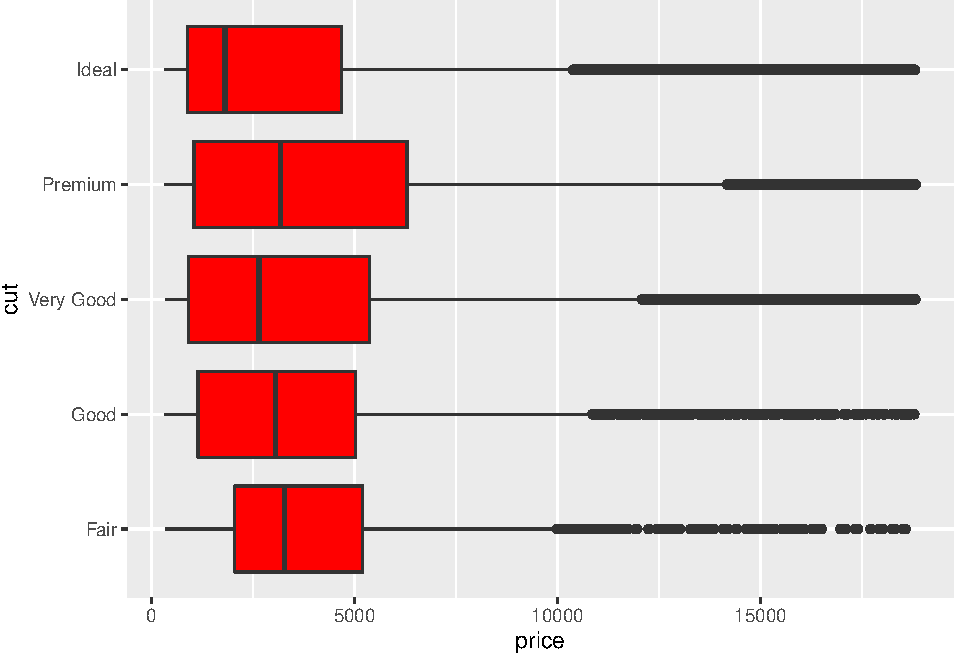
\includegraphics[width=0.75\linewidth]{Lab4_files/figure-latex/unnamed-chunk-5-1} 

}

\caption{Precio vrs. corte.}\label{fig:unnamed-chunk-5}
\end{figure}

\hypertarget{precio-vrs.-peso}{%
\subsection{Precio vrs. peso}\label{precio-vrs.-peso}}

\begin{verbatim}
## Warning: Continuous x aesthetic -- did you forget aes(group=...)?
\end{verbatim}

\begin{figure}[H]

{\centering 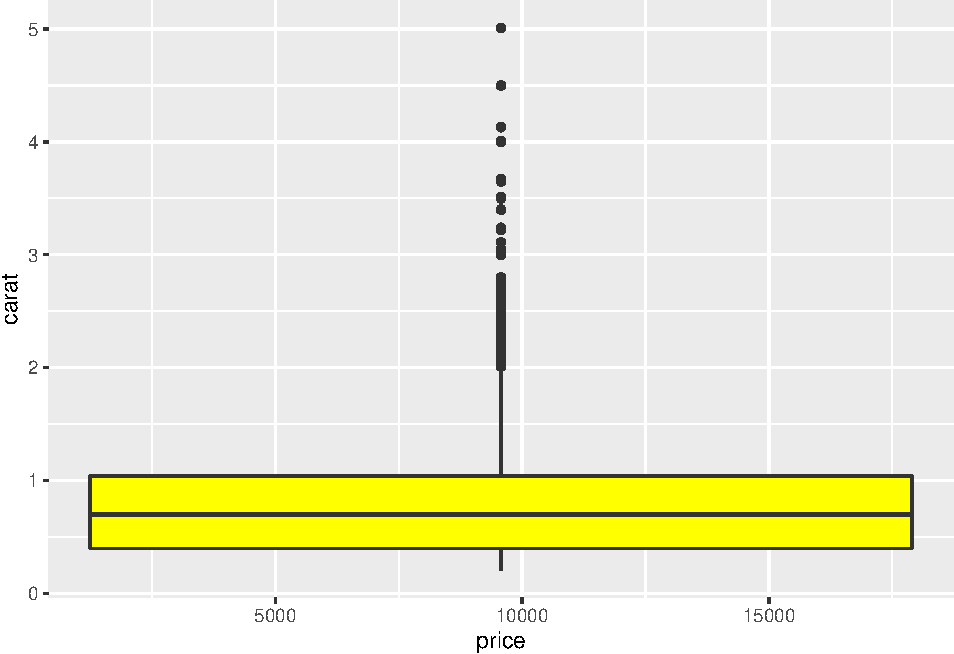
\includegraphics[width=0.75\linewidth]{Lab4_files/figure-latex/unnamed-chunk-6-1} 

}

\caption{Precio vrs. peso.}\label{fig:unnamed-chunk-6}
\end{figure}

\hypertarget{precio-vrs.-claridad}{%
\subsection{Precio vrs. claridad}\label{precio-vrs.-claridad}}

\begin{figure}[H]

{\centering 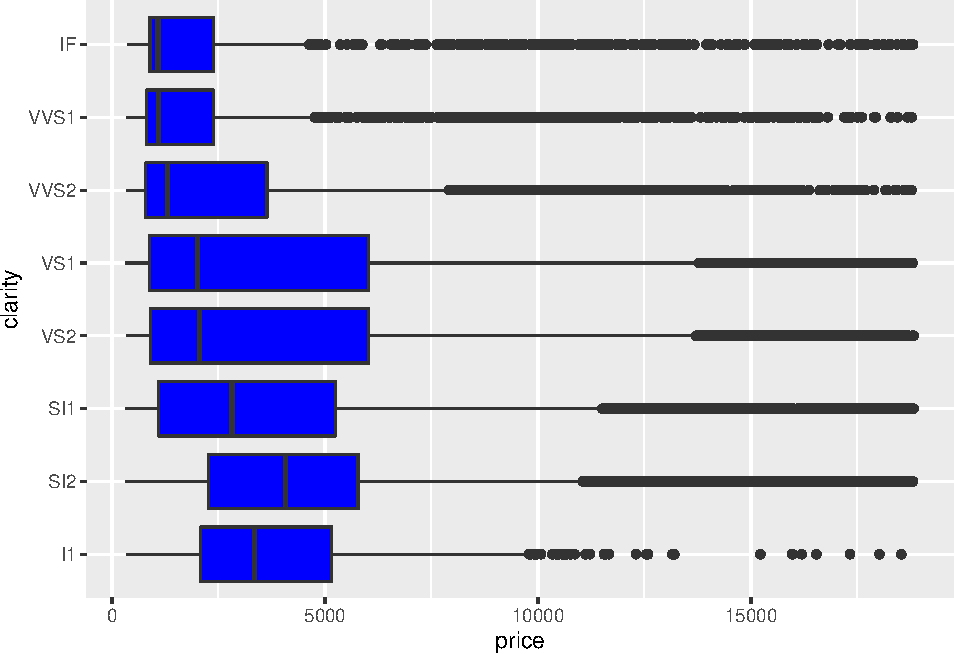
\includegraphics[width=0.75\linewidth]{Lab4_files/figure-latex/unnamed-chunk-7-1} 

}

\caption{Precio vrs. claridad.}\label{fig:unnamed-chunk-7}
\end{figure}

La interpretación de las cajas de bigote parecieran indicar que existen una cantidad excesiva de puntos atípicos, por lo tanto, en una regresión lineal mucho más detallada; sería necesario eliminarlos para obtener mejores resultados. 

\hypertarget{haga-una-matriz-de-correlaciuxf3n-y-analice-los-resultados.-hay-alguna-variable-que-estuxe9-altamente-relacionada}{%
\section{Haga una matriz de correlación y analice los resultados. ¿Hay
alguna variable que esté altamente
relacionada?}\label{haga-una-matriz-de-correlaciuxf3n-y-analice-los-resultados.-hay-alguna-variable-que-estuxe9-altamente-relacionada}}

\begin{Shaded}
\begin{Highlighting}[]
\CommentTok{#Evaluar que columnas son numéricas}
\NormalTok{vect_num <-}\StringTok{ }\KeywordTok{sapply}\NormalTok{(diamonds, is.numeric)}
\CommentTok{#Vector de valores lógicos para filtrar numéricos}
\NormalTok{cor_diamonds <-}\StringTok{ }\KeywordTok{cor}\NormalTok{(diamonds[,vect_num])}
\CommentTok{#Graficar}
\KeywordTok{corrplot}\NormalTok{(cor_diamonds,}\DataTypeTok{method =} \StringTok{"number"}\NormalTok{, }\DataTypeTok{sig.level=}\FloatTok{0.05}\NormalTok{)}
\end{Highlighting}
\end{Shaded}

\begin{figure}[H]

{\centering 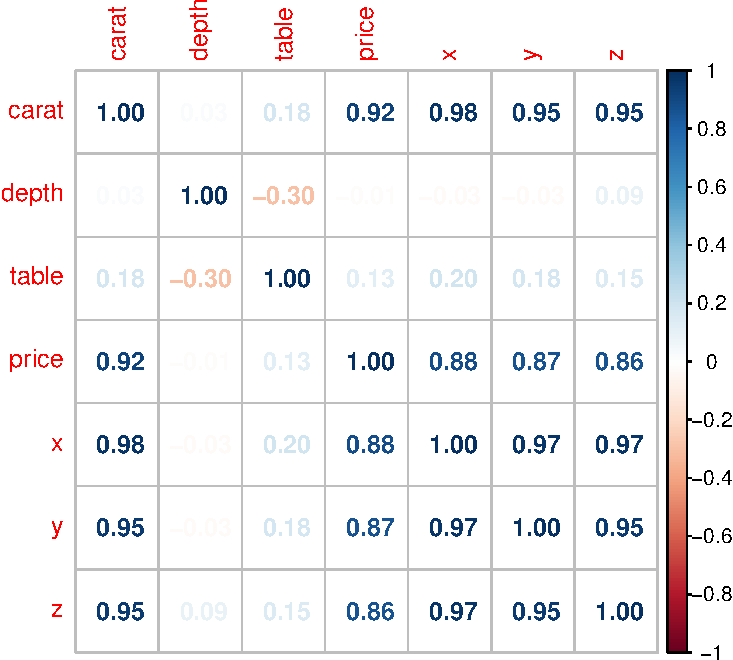
\includegraphics[width=0.75\linewidth]{Lab4_files/figure-latex/unnamed-chunk-8-1} 

}

\caption{Matriz de correlación}\label{fig:unnamed-chunk-8}
\end{figure}

\begin{Shaded}
\begin{Highlighting}[]
\KeywordTok{help}\NormalTok{(corrplot)}
\end{Highlighting}
\end{Shaded}

Las relaciones significativas son las siguientes:

\begin{enumerate}
  \item carat con price,x,y,z. 
  \item price con carat,x,y,z.
\end{enumerate}

\hypertarget{haga-la-particiuxf3n-de-datos-en-entrenamiento-y-prueba.}{%
\section{Haga la partición de datos en entrenamiento y
prueba.}\label{haga-la-particiuxf3n-de-datos-en-entrenamiento-y-prueba.}}

\begin{Shaded}
\begin{Highlighting}[]
\KeywordTok{library}\NormalTok{(caTools)}
\end{Highlighting}
\end{Shaded}

\begin{Shaded}
\begin{Highlighting}[]
\CommentTok{# Fijamos la aleatoriedad }
\KeywordTok{set.seed}\NormalTok{(}\DecValTok{69}\NormalTok{)}
\CommentTok{#Partición de los datos}
\NormalTok{muestreo <-}\StringTok{ }\KeywordTok{sample.split}\NormalTok{(diamonds}\OperatorTok{$}\NormalTok{price, }\DataTypeTok{SplitRatio =} \FloatTok{0.7}\NormalTok{)}
\CommentTok{# Los subconjuntos de datos entrenamiento y prueba}
\NormalTok{entrenamiento <-}\StringTok{ }\KeywordTok{subset}\NormalTok{(diamonds, muestreo }\OperatorTok{==}\StringTok{ }\NormalTok{T)}
\NormalTok{prueba <-}\StringTok{ }\KeywordTok{subset}\NormalTok{(diamonds, muestreo }\OperatorTok{==}\StringTok{ }\NormalTok{F)}
\end{Highlighting}
\end{Shaded}

\hypertarget{entrene-el-modelo-de-regresiuxf3n-lineal-usando-todas-las-variables-como-predictoras.}{%
\section{Entrene el modelo de regresión lineal usando todas las
variables como
predictoras.}\label{entrene-el-modelo-de-regresiuxf3n-lineal-usando-todas-las-variables-como-predictoras.}}

\begin{Shaded}
\begin{Highlighting}[]
\NormalTok{modelo <-}\StringTok{ }\KeywordTok{lm}\NormalTok{(price }\OperatorTok{~}\StringTok{ }\NormalTok{.,entrenamiento)}
\KeywordTok{summary}\NormalTok{(modelo)}
\end{Highlighting}
\end{Shaded}

\begin{verbatim}
## 
## Call:
## lm(formula = price ~ ., data = entrenamiento)
## 
## Residuals:
##      Min       1Q   Median       3Q      Max 
## -21396.7   -621.3   -192.9    396.2  10537.9 
## 
## Coefficients:
##              Estimate Std. Error t value Pr(>|t|)    
## (Intercept)  5481.993    543.114  10.094  < 2e-16 ***
## carat       11280.437     58.662 192.294  < 2e-16 ***
## cut.L         592.607     27.741  21.362  < 2e-16 ***
## cut.Q        -305.994     22.246 -13.755  < 2e-16 ***
## cut.C         150.618     18.962   7.943 2.03e-15 ***
## cut^4         -20.724     15.193  -1.364  0.17255    
## color.L     -2043.221     21.202 -96.370  < 2e-16 ***
## color.Q      -692.693     19.276 -35.935  < 2e-16 ***
## color.C      -177.222     18.012  -9.839  < 2e-16 ***
## color^4        35.826     16.582   2.161  0.03074 *  
## color^5      -107.147     15.669  -6.838 8.15e-12 ***
## color^6       -40.671     14.263  -2.851  0.00435 ** 
## clarity.L    4234.218     37.148 113.982  < 2e-16 ***
## clarity.Q   -1965.189     34.687 -56.655  < 2e-16 ***
## clarity.C    1010.730     29.720  34.009  < 2e-16 ***
## clarity^4    -373.315     23.733 -15.730  < 2e-16 ***
## clarity^5     257.064     19.394  13.255  < 2e-16 ***
## clarity^6       4.514     16.878   0.267  0.78914    
## clarity^7     103.048     14.869   6.930 4.27e-12 ***
## depth         -60.021      6.770  -8.866  < 2e-16 ***
## table         -28.555      3.584  -7.967 1.66e-15 ***
## x            -907.544     51.372 -17.666  < 2e-16 ***
## y               8.096     20.744   0.390  0.69633    
## z            -168.213     75.499  -2.228  0.02588 *  
## ---
## Signif. codes:  0 '***' 0.001 '**' 0.01 '*' 0.05 '.' 0.1 ' ' 1
## 
## Residual standard error: 1172 on 38453 degrees of freedom
## Multiple R-squared:  0.9196, Adjusted R-squared:  0.9195 
## F-statistic: 1.912e+04 on 23 and 38453 DF,  p-value: < 2.2e-16
\end{verbatim}

\begin{Shaded}
\begin{Highlighting}[]
\NormalTok{predicciones <-}\StringTok{ }\KeywordTok{predict}\NormalTok{(modelo, prueba)}
\NormalTok{resultados <-}\StringTok{ }\KeywordTok{cbind}\NormalTok{(prueba, predicciones)}
\KeywordTok{kbl}\NormalTok{(}\KeywordTok{head}\NormalTok{(resultados), }\DataTypeTok{booktabs =}\NormalTok{ T) }\OperatorTok\StringTok{ }\KeywordTok{kable_styling}\NormalTok{(}\DataTypeTok{latex_options =} 
                                               \KeywordTok{c}\NormalTok{(}\StringTok{"striped"}\NormalTok{,}\StringTok{"scale_down"}\NormalTok{, }\StringTok{"hold_position"}\NormalTok{))}
\end{Highlighting}
\end{Shaded}

\begin{table}[!h]
\centering
\resizebox{\linewidth}{!}{
\begin{tabular}[t]{rlllrrrrrrr}
\toprule
carat & cut & color & clarity & depth & table & price & x & y & z & predicciones\\
\midrule
\cellcolor{gray!6}{0.21} & \cellcolor{gray!6}{Premium} & \cellcolor{gray!6}{E} & \cellcolor{gray!6}{SI1} & \cellcolor{gray!6}{59.8} & \cellcolor{gray!6}{61} & \cellcolor{gray!6}{326} & \cellcolor{gray!6}{3.89} & \cellcolor{gray!6}{3.84} & \cellcolor{gray!6}{2.31} & \cellcolor{gray!6}{-715.8744}\\
0.24 & Very Good & J & VVS2 & 62.8 & 57 & 336 & 3.94 & 3.96 & 2.48 & -1455.3399\\
\cellcolor{gray!6}{0.26} & \cellcolor{gray!6}{Very Good} & \cellcolor{gray!6}{H} & \cellcolor{gray!6}{SI1} & \cellcolor{gray!6}{61.9} & \cellcolor{gray!6}{55} & \cellcolor{gray!6}{337} & \cellcolor{gray!6}{4.07} & \cellcolor{gray!6}{4.11} & \cellcolor{gray!6}{2.53} & \cellcolor{gray!6}{-1143.5258}\\
0.32 & Premium & E & I1 & 60.9 & 58 & 345 & 4.38 & 4.42 & 2.68 & -3713.8419\\
\cellcolor{gray!6}{0.30} & \cellcolor{gray!6}{Very Good} & \cellcolor{gray!6}{J} & \cellcolor{gray!6}{SI1} & \cellcolor{gray!6}{62.7} & \cellcolor{gray!6}{59} & \cellcolor{gray!6}{351} & \cellcolor{gray!6}{4.21} & \cellcolor{gray!6}{4.27} & \cellcolor{gray!6}{2.66} & \cellcolor{gray!6}{-2452.5050}\\
\addlinespace
0.23 & Very Good & H & VS1 & 61.0 & 57 & 353 & 3.94 & 3.96 & 2.41 & -393.1858\\
\bottomrule
\end{tabular}}
\end{table}

\hypertarget{haga-una-funciuxf3n-que-diga-si-el-resultado-es-negativo-debe-colocar-el-valor-muxednimo-de-precio-dentro-de-la-base-de-datos.}{%
\section{Haga una función que diga si el resultado es negativo, debe
colocar el valor mínimo de precio dentro de la base de
datos.}\label{haga-una-funciuxf3n-que-diga-si-el-resultado-es-negativo-debe-colocar-el-valor-muxednimo-de-precio-dentro-de-la-base-de-datos.}}

\begin{Shaded}
\begin{Highlighting}[]
\NormalTok{convertir_cero <-}\StringTok{ }\ControlFlowTok{function}\NormalTok{(x)\{}
  \ControlFlowTok{if}\NormalTok{(x}\OperatorTok{<}\DecValTok{0}\NormalTok{)\{}
    \KeywordTok{return}\NormalTok{ (}\KeywordTok{min}\NormalTok{(diamonds}\OperatorTok{$}\NormalTok{price))}
\NormalTok{  \} }\ControlFlowTok{else}\NormalTok{\{}
    \KeywordTok{return}\NormalTok{ (x)}
\NormalTok{  \}}
\NormalTok{\}}
\end{Highlighting}
\end{Shaded}

\hypertarget{corra-la-funciuxf3n-con-las-predicciones.}{%
\section{Corra la función con las
predicciones.}\label{corra-la-funciuxf3n-con-las-predicciones.}}

\begin{Shaded}
\begin{Highlighting}[]
\NormalTok{resultados}\OperatorTok{$}\NormalTok{predicciones <-}\StringTok{ }\KeywordTok{sapply}\NormalTok{(resultados}\OperatorTok{$}\NormalTok{predicciones, convertir_cero)}

\KeywordTok{kbl}\NormalTok{(}\KeywordTok{head}\NormalTok{(resultados), }\DataTypeTok{booktabs =}\NormalTok{ T) }\OperatorTok\StringTok{ }\KeywordTok{kable_styling}\NormalTok{(}\DataTypeTok{latex_options =} 
                                               \KeywordTok{c}\NormalTok{(}\StringTok{"striped"}\NormalTok{,}\StringTok{"scale_down"}\NormalTok{, }\StringTok{"hold_position"}\NormalTok{))}
\end{Highlighting}
\end{Shaded}

\begin{table}[!h]
\centering
\resizebox{\linewidth}{!}{
\begin{tabular}[t]{rlllrrrrrrr}
\toprule
carat & cut & color & clarity & depth & table & price & x & y & z & predicciones\\
\midrule
\cellcolor{gray!6}{0.21} & \cellcolor{gray!6}{Premium} & \cellcolor{gray!6}{E} & \cellcolor{gray!6}{SI1} & \cellcolor{gray!6}{59.8} & \cellcolor{gray!6}{61} & \cellcolor{gray!6}{326} & \cellcolor{gray!6}{3.89} & \cellcolor{gray!6}{3.84} & \cellcolor{gray!6}{2.31} & \cellcolor{gray!6}{326}\\
0.24 & Very Good & J & VVS2 & 62.8 & 57 & 336 & 3.94 & 3.96 & 2.48 & 326\\
\cellcolor{gray!6}{0.26} & \cellcolor{gray!6}{Very Good} & \cellcolor{gray!6}{H} & \cellcolor{gray!6}{SI1} & \cellcolor{gray!6}{61.9} & \cellcolor{gray!6}{55} & \cellcolor{gray!6}{337} & \cellcolor{gray!6}{4.07} & \cellcolor{gray!6}{4.11} & \cellcolor{gray!6}{2.53} & \cellcolor{gray!6}{326}\\
0.32 & Premium & E & I1 & 60.9 & 58 & 345 & 4.38 & 4.42 & 2.68 & 326\\
\cellcolor{gray!6}{0.30} & \cellcolor{gray!6}{Very Good} & \cellcolor{gray!6}{J} & \cellcolor{gray!6}{SI1} & \cellcolor{gray!6}{62.7} & \cellcolor{gray!6}{59} & \cellcolor{gray!6}{351} & \cellcolor{gray!6}{4.21} & \cellcolor{gray!6}{4.27} & \cellcolor{gray!6}{2.66} & \cellcolor{gray!6}{326}\\
\addlinespace
0.23 & Very Good & H & VS1 & 61.0 & 57 & 353 & 3.94 & 3.96 & 2.41 & 326\\
\bottomrule
\end{tabular}}
\end{table}

\hypertarget{cuuxe1l-es-el-mape-del-modelo-cuuxe1l-es-el-rmse-del-modelo-estuxe1-haciendo-un-buen-trabajo-el-modelo}{%
\section{¿Cuál es el MAPE del modelo? ¿Cuál es el RMSE del modelo? ¿Está
haciendo un buen trabajo el
modelo?}\label{cuuxe1l-es-el-mape-del-modelo-cuuxe1l-es-el-rmse-del-modelo-estuxe1-haciendo-un-buen-trabajo-el-modelo}}

\begin{Shaded}
\begin{Highlighting}[]
\NormalTok{MAPE <-}\StringTok{ }\DecValTok{100}\OperatorTok{/}\KeywordTok{nrow}\NormalTok{(resultados)}\OperatorTok{*}\StringTok{ }\KeywordTok{sum}\NormalTok{((resultados}\OperatorTok{$}\NormalTok{price}\OperatorTok{-}\NormalTok{resultados}\OperatorTok{$}\NormalTok{predicciones)}\OperatorTok{/}\NormalTok{resultados}\OperatorTok{$}\NormalTok{price)}
\NormalTok{MAPE}
\end{Highlighting}
\end{Shaded}

\begin{verbatim}
## [1] -6.234558
\end{verbatim}

\begin{Shaded}
\begin{Highlighting}[]
\NormalTok{MSE <-}\StringTok{ }\KeywordTok{mean}\NormalTok{((resultados}\OperatorTok{$}\NormalTok{price }\OperatorTok{-}\StringTok{ }\NormalTok{resultados}\OperatorTok{$}\NormalTok{predicciones)}\OperatorTok{^}\DecValTok{2}\NormalTok{)}
\NormalTok{RMSE <-}\StringTok{ }\KeywordTok{sqrt}\NormalTok{(MSE)}
\NormalTok{RMSE}
\end{Highlighting}
\end{Shaded}

\begin{verbatim}
## [1] 949.8472
\end{verbatim}

Los resultados encontrados en el MAPE y indican un porcentaje negativo
de aproximadamente -6\% comparado entre los precios reales y las
prediciones; por otra parte el RMSE indica una pérdida muy pequeña. Por
lo tanto, el modelo está haciendo un buen trabajo.

\hypertarget{utilice-el-modelo-para-hacer-las-proyecciones-utilizando-el-archivo-de-diamantes---uso.csv.}{%
\section{Utilice el modelo para hacer las proyecciones utilizando el
archivo de ``diamantes -
uso.csv''.}\label{utilice-el-modelo-para-hacer-las-proyecciones-utilizando-el-archivo-de-diamantes---uso.csv.}}

\begin{Shaded}
\begin{Highlighting}[]
\KeywordTok{getwd}\NormalTok{()}
\end{Highlighting}
\end{Shaded}

\begin{verbatim}
## [1] "/Users/rudiks/Git/UVG-DataMining-Notas-6-Semestre/Laboratorio4"
\end{verbatim}

\begin{Shaded}
\begin{Highlighting}[]
\NormalTok{uso <-}\StringTok{ }\KeywordTok{read.csv}\NormalTok{(}\StringTok{"diamantes - uso.csv"}\NormalTok{, }\DataTypeTok{sep =} \StringTok{";"}\NormalTok{)}
\NormalTok{predicciones_uso <-}\StringTok{ }\KeywordTok{predict}\NormalTok{(modelo, uso)}
\NormalTok{resultados_uso <-}\StringTok{ }\KeywordTok{cbind}\NormalTok{(uso, predicciones_uso)}
\NormalTok{resultados_uso}\OperatorTok{$}\NormalTok{predicciones_uso <-}\StringTok{ }\KeywordTok{sapply}\NormalTok{(resultados_uso}\OperatorTok{$}\NormalTok{predicciones_uso, convertir_cero)}
\KeywordTok{kbl}\NormalTok{(}\KeywordTok{head}\NormalTok{(resultados_uso, }\DecValTok{30}\NormalTok{), }\DataTypeTok{booktabs =}\NormalTok{ T) }\OperatorTok\StringTok{ }\KeywordTok{kable_styling}\NormalTok{(}\DataTypeTok{latex_options =} 
                                               \KeywordTok{c}\NormalTok{(}\StringTok{"striped"}\NormalTok{,}\StringTok{"scale_down"}\NormalTok{, }\StringTok{"hold_position"}\NormalTok{))}
\end{Highlighting}
\end{Shaded}

\begin{table}[!h]
\centering
\resizebox{\linewidth}{!}{
\begin{tabular}[t]{rlllrrrrrr}
\toprule
carat & cut & color & clarity & depth & table & x & y & z & predicciones\_uso\\
\midrule
\cellcolor{gray!6}{0.32} & \cellcolor{gray!6}{Ideal} & \cellcolor{gray!6}{I} & \cellcolor{gray!6}{VVS1} & \cellcolor{gray!6}{62.0} & \cellcolor{gray!6}{55.3} & \cellcolor{gray!6}{4.39} & \cellcolor{gray!6}{4.42} & \cellcolor{gray!6}{2.73} & \cellcolor{gray!6}{200.84299}\\
0.31 & Very Good & G & SI1 & 63.3 & 57.0 & 4.33 & 4.30 & 2.73 & 326.00000\\
\cellcolor{gray!6}{0.31} & \cellcolor{gray!6}{Premium} & \cellcolor{gray!6}{G} & \cellcolor{gray!6}{SI1} & \cellcolor{gray!6}{61.8} & \cellcolor{gray!6}{58.0} & \cellcolor{gray!6}{4.35} & \cellcolor{gray!6}{4.32} & \cellcolor{gray!6}{2.68} & \cellcolor{gray!6}{326.00000}\\
0.24 & Premium & E & VVS1 & 60.7 & 58.0 & 4.01 & 4.03 & 2.44 & 923.56890\\
\cellcolor{gray!6}{0.24} & \cellcolor{gray!6}{Very Good} & \cellcolor{gray!6}{D} & \cellcolor{gray!6}{VVS1} & \cellcolor{gray!6}{61.5} & \cellcolor{gray!6}{60.0} & \cellcolor{gray!6}{3.97} & \cellcolor{gray!6}{4.00} & \cellcolor{gray!6}{2.45} & \cellcolor{gray!6}{1048.58370}\\
\addlinespace
0.30 & Very Good & H & SI1 & 63.1 & 56.0 & 4.29 & 4.27 & 2.70 & 326.00000\\
\cellcolor{gray!6}{0.30} & \cellcolor{gray!6}{Premium} & \cellcolor{gray!6}{H} & \cellcolor{gray!6}{SI1} & \cellcolor{gray!6}{62.9} & \cellcolor{gray!6}{59.0} & \cellcolor{gray!6}{4.28} & \cellcolor{gray!6}{4.24} & \cellcolor{gray!6}{2.68} & \cellcolor{gray!6}{326.00000}\\
0.30 & Premium & H & SI1 & 62.5 & 57.0 & 4.29 & 4.25 & 2.67 & 326.00000\\
\cellcolor{gray!6}{0.30} & \cellcolor{gray!6}{Good} & \cellcolor{gray!6}{H} & \cellcolor{gray!6}{SI1} & \cellcolor{gray!6}{63.7} & \cellcolor{gray!6}{57.0} & \cellcolor{gray!6}{4.28} & \cellcolor{gray!6}{4.26} & \cellcolor{gray!6}{2.72} & \cellcolor{gray!6}{326.00000}\\
0.26 & Very Good & F & VVS2 & 59.2 & 60.0 & 4.19 & 4.22 & 2.49 & 869.01722\\
\addlinespace
\cellcolor{gray!6}{0.26} & \cellcolor{gray!6}{Very Good} & \cellcolor{gray!6}{E} & \cellcolor{gray!6}{VVS2} & \cellcolor{gray!6}{59.9} & \cellcolor{gray!6}{58.0} & \cellcolor{gray!6}{4.15} & \cellcolor{gray!6}{4.23} & \cellcolor{gray!6}{2.51} & \cellcolor{gray!6}{976.31288}\\
0.26 & Very Good & D & VVS2 & 62.4 & 54.0 & 4.08 & 4.13 & 2.56 & 1225.68413\\
\cellcolor{gray!6}{0.26} & \cellcolor{gray!6}{Very Good} & \cellcolor{gray!6}{D} & \cellcolor{gray!6}{VVS2} & \cellcolor{gray!6}{62.8} & \cellcolor{gray!6}{60.0} & \cellcolor{gray!6}{4.01} & \cellcolor{gray!6}{4.05} & \cellcolor{gray!6}{2.53} & \cellcolor{gray!6}{1098.26967}\\
0.26 & Very Good & E & VVS1 & 62.6 & 59.0 & 4.06 & 4.09 & 2.55 & 908.05723\\
\cellcolor{gray!6}{0.26} & \cellcolor{gray!6}{Very Good} & \cellcolor{gray!6}{E} & \cellcolor{gray!6}{VVS1} & \cellcolor{gray!6}{63.4} & \cellcolor{gray!6}{59.0} & \cellcolor{gray!6}{4.00} & \cellcolor{gray!6}{4.04} & \cellcolor{gray!6}{2.55} & \cellcolor{gray!6}{914.08788}\\
\addlinespace
0.26 & Very Good & D & VVS1 & 62.1 & 60.0 & 4.03 & 4.12 & 2.53 & 1171.24140\\
\cellcolor{gray!6}{0.26} & \cellcolor{gray!6}{Ideal} & \cellcolor{gray!6}{E} & \cellcolor{gray!6}{VVS2} & \cellcolor{gray!6}{62.9} & \cellcolor{gray!6}{58.0} & \cellcolor{gray!6}{4.02} & \cellcolor{gray!6}{4.06} & \cellcolor{gray!6}{2.54} & \cellcolor{gray!6}{1015.49743}\\
0.38 & Ideal & I & SI2 & 61.6 & 56.0 & 4.65 & 4.67 & 2.87 & 326.00000\\
\cellcolor{gray!6}{0.26} & \cellcolor{gray!6}{Good} & \cellcolor{gray!6}{E} & \cellcolor{gray!6}{VVS1} & \cellcolor{gray!6}{57.9} & \cellcolor{gray!6}{60.0} & \cellcolor{gray!6}{4.22} & \cellcolor{gray!6}{4.25} & \cellcolor{gray!6}{2.45} & \cellcolor{gray!6}{885.36310}\\
0.24 & Premium & G & VVS1 & 62.3 & 59.0 & 3.95 & 3.92 & 2.45 & 556.28487\\
\addlinespace
\cellcolor{gray!6}{0.24} & \cellcolor{gray!6}{Premium} & \cellcolor{gray!6}{H} & \cellcolor{gray!6}{VVS1} & \cellcolor{gray!6}{61.2} & \cellcolor{gray!6}{58.0} & \cellcolor{gray!6}{4.01} & \cellcolor{gray!6}{3.96} & \cellcolor{gray!6}{2.44} & \cellcolor{gray!6}{89.33879}\\
0.24 & Premium & H & VVS1 & 60.8 & 59.0 & 4.02 & 4.00 & 2.44 & 76.04035\\
\cellcolor{gray!6}{0.24} & \cellcolor{gray!6}{Premium} & \cellcolor{gray!6}{H} & \cellcolor{gray!6}{VVS2} & \cellcolor{gray!6}{60.7} & \cellcolor{gray!6}{58.0} & \cellcolor{gray!6}{4.07} & \cellcolor{gray!6}{4.04} & \cellcolor{gray!6}{2.46} & \cellcolor{gray!6}{13.63949}\\
0.32 & Premium & I & SI1 & 62.9 & 58.0 & 4.35 & 4.33 & 2.73 & 326.00000\\
\cellcolor{gray!6}{0.70} & \cellcolor{gray!6}{Ideal} & \cellcolor{gray!6}{E} & \cellcolor{gray!6}{SI1} & \cellcolor{gray!6}{62.5} & \cellcolor{gray!6}{57.0} & \cellcolor{gray!6}{5.70} & \cellcolor{gray!6}{5.72} & \cellcolor{gray!6}{3.57} & \cellcolor{gray!6}{2996.88262}\\
\addlinespace
0.86 & Fair & E & SI2 & 55.1 & 69.0 & 6.45 & 6.33 & 3.52 & 2422.64877\\
\cellcolor{gray!6}{0.70} & \cellcolor{gray!6}{Ideal} & \cellcolor{gray!6}{G} & \cellcolor{gray!6}{VS2} & \cellcolor{gray!6}{61.6} & \cellcolor{gray!6}{56.0} & \cellcolor{gray!6}{5.70} & \cellcolor{gray!6}{5.67} & \cellcolor{gray!6}{3.50} & \cellcolor{gray!6}{3429.13881}\\
0.71 & Very Good & E & VS2 & 62.4 & 57.0 & 5.68 & 5.73 & 3.56 & 3660.79754\\
\cellcolor{gray!6}{0.78} & \cellcolor{gray!6}{Very Good} & \cellcolor{gray!6}{G} & \cellcolor{gray!6}{SI2} & \cellcolor{gray!6}{63.8} & \cellcolor{gray!6}{56.0} & \cellcolor{gray!6}{5.81} & \cellcolor{gray!6}{5.85} & \cellcolor{gray!6}{3.72} & \cellcolor{gray!6}{2355.13596}\\
0.70 & Good & E & VS2 & 57.5 & 58.0 & 5.85 & 5.90 & 3.38 & 3541.76590\\
\bottomrule
\end{tabular}}
\end{table}

\end{document}
